\documentclass{article}%
\usepackage[T1]{fontenc}%
\usepackage[utf8]{inputenc}%
\usepackage{lmodern}%
\usepackage{textcomp}%
\usepackage{lastpage}%
\usepackage[head=40pt,margin=0.5in,bottom=0.6in]{geometry}%
\usepackage{graphicx}%
%
\title{\textbf{Aumentan la minería ilegal y el paludismo en Amazonas}}%
\author{El Nacional Web}%
\date{09/10/2018}%
%
\begin{document}%
\normalsize%
\maketitle%
\textbf{URL: }%
http://www.el{-}nacional.com/noticias/salud/aumentan{-}mineria{-}ilegal{-}paludismo{-}amazonas\_254975\newline%
%
\textbf{Periodico: }%
EN, %
ID: %
254975, %
Seccion: %
Salud\newline%
%
\textbf{Palabras Claves: }%
Salud, Medicinas, Gobierno\newline%
%
\textbf{Derecho: }%
3.2, %
Otros Derechos: %
2.1, %
Sub Derechos: %
3.2.1, 2.1.1\newline%
%
\textbf{EP: }%
NO\newline%
\newline%
%
\textbf{\textit{De acuerdo con data oficial de la Dirección de Salud Ambiental del Ministerio de Salud, durante el primer trimestre de 2018 se confirmaron~797 casos de malaria}}%
\newline%
\newline%
%
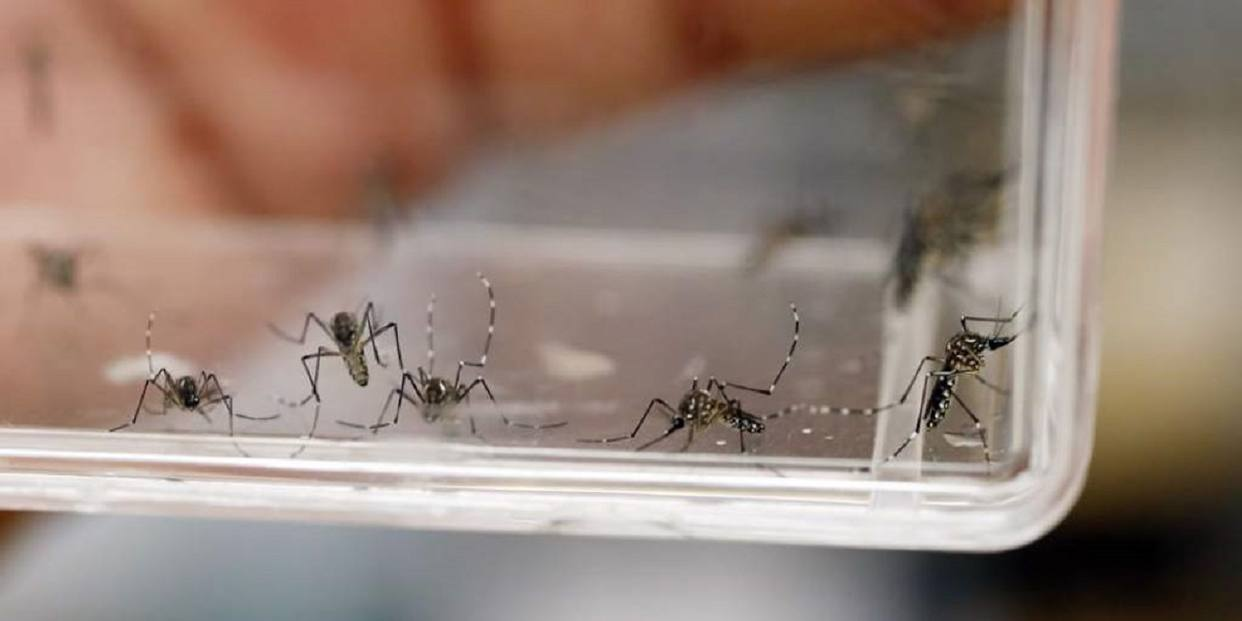
\includegraphics[width=300px]{101.jpg}%
\newline%
%
El Observatorio de Derechos Indígenas~Kapé Kapé~hizo seguimiento a la~situación sanitaria~en~Amazonas. En la entidad se investigó sobre los impactos socioambientales~de la minería ilegal, reseñó~El Pitazo.%
\newline%
%
“El Alto Orinoco es uno de los más perjudicados por la minería ilegal, presentando altos casos de~paludismo~de todos los niveles, de acuerdo con lo que indican los números porcentuales de su densidad poblacional”, explicó Luis Betancourt, principal investigador de la organización.%
\newline%
%
Un balance de la organización Kapé~Kapé,~el Alto Orinoco presentó~396 casos entre 11.000 habitantes.~En el municipio Manapiare, según data oficial de la Dirección de Salud Ambiental del Ministerio de Salud, durante el primer trimestre de 2018 se confirmaron~797 casos de malaria.%
\newline%
%
Wilmer Pérez, promotor social del referido sector,~explicó que padecen una difícil y grave situación sanitaria, en especial con la malaria y~desnutrición infantil.%
\newline%
%
Lea más en~El Pitazo.%
\newline%
%
\end{document}